% =============================================================
% CS495 -- Data Science Project Practicum
% Capstone Poster -- Bellevue College
% "Mapping Best Empirical Models: A Meta-Analysis of Winning
%  Kaggle Tabular Solutions" -- Kenneth Young
%
% Built from the official BC poster template (private/bellevuecollegetemplate.tex);
% visual system (a0poster class, BC colors, posterblock/callout styles, banner,
% footer) is unchanged. Only content is project-specific.
%
% Compile: pdflatex poster.tex (run twice). Place
% BellevueCollegeLogoHorzClr.png next to this file. Figures are pulled from
% ../report/figures/ via \graphicspath.
% =============================================================

\documentclass[a0,portrait]{a0poster}

% ---------- Packages ----------
\usepackage[utf8]{inputenc}
\usepackage[T1]{fontenc}
\usepackage[english]{babel}
\usepackage{graphicx}
\usepackage{amsmath,amssymb}
\usepackage{booktabs}
\usepackage{array}
\usepackage{multicol}
\usepackage{xcolor}
\usepackage{enumitem}
\usepackage{tcolorbox}
\usepackage{tikz}
\usepackage{ragged2e}
\usepackage{anyfontsize}
\tcbuselibrary{skins,breakable}
\usetikzlibrary{arrows.meta, positioning, fit, backgrounds, decorations.pathreplacing}

\graphicspath{{../report/figures/}{./}}

% ---------- Bellevue College Brand Colors ----------
\definecolor{BCBlue}{HTML}{003D79}        % Brutus Blue   (primary)
\definecolor{BCSilver}{HTML}{A7A9AC}      % Bulldog Silver (primary)
\definecolor{BCRed}{HTML}{C4122F}         % Fall Maple Red (accent)
\definecolor{BCLightBlue}{HTML}{E6EEF7}   % Soft tinted background
\definecolor{BCDarkBlue}{HTML}{002851}    % Deeper variant
\definecolor{BCInk}{HTML}{1A1A1A}         % Body text

% ---------- Layout ----------
\setlength{\parindent}{0pt}
\setlength{\parskip}{0.5em}
\setlength{\columnsep}{2.5cm}
\setlength{\columnseprule}{0pt}

% ---------- Block container ----------
\newtcolorbox{posterblock}[1]{
    enhanced, breakable, before upper={\raggedright},
    colback=white, colframe=BCSilver,
    boxrule=0.8pt, arc=6pt,
    left=18pt, right=18pt, top=10pt, bottom=14pt,
    fonttitle=\bfseries\Large,
    title={#1},
    coltitle=white,
    colbacktitle=BCBlue,
    attach boxed title to top left={xshift=0mm, yshift=0mm},
    boxed title style={
        colback=BCBlue, colframe=BCBlue,
        sharp corners, boxrule=0pt,
        left=14pt, right=18pt, top=8pt, bottom=8pt,
    },
    title filled=true,
    before skip=18pt, after skip=18pt,
    overlay unbroken and first={
        \fill[BCRed] (frame.north west) rectangle ([xshift=12pt]frame.north west|-title.south);
    },
}

% ---------- Inline tinted callout box ----------
\newtcolorbox{callout}{
    colback=BCLightBlue, colframe=BCLightBlue,
    arc=4pt, left=14pt, right=14pt, top=10pt, bottom=10pt,
    boxrule=0pt,
}

% ---------- Figure caption helper ----------
\newcommand{\figcap}[1]{\par\vspace{0.2em}{\small\itshape\color{BCDarkBlue}#1}}

\begin{document}

% =============================================================
% TITLE BANNER
% =============================================================
\noindent

\begin{tikzpicture}[remember picture]
  \fill[BCLightBlue] (0,0) rectangle (\textwidth, 11cm);
  \fill[BCRed]  (0,0) rectangle (\textwidth, 0.6cm);

  % Logo on the left
  \node[anchor=west, inner sep=0pt] at (1cm, 6cm) {
    \IfFileExists{BellevueCollegeLogoHorzClr.png}{%
      \includegraphics[height=7cm]{BellevueCollegeLogoHorzClr.png}%
    }{%
      \colorbox{BCDarkBlue}{\parbox[c][7cm][c]{22cm}{\centering\bfseries\color{BCBlue}\fontsize{50}{60}\selectfont
        Bellevue College\\[6pt]\fontsize{22}{26}\selectfont\itshape (place logo here)}}%
    }
  };

  % Title text on the right
  \node[anchor=west, inner sep=0pt, text width=\textwidth-32cm, align=left]
       at (32cm, 7.8cm) {%
    \color{BCDarkBlue}\fontsize{64}{74}\selectfont\bfseries
    Mapping Best Empirical Models
  };
  \node[anchor=west, inner sep=0pt, text width=\textwidth-32cm, align=left]
       at (32cm, 4.9cm) {%
    \color{BCBlue}\fontsize{38}{46}\selectfont\bfseries
    A Meta-Analysis of Winning Kaggle Tabular Solutions
  };
  \node[anchor=west, inner sep=0pt, text width=\textwidth-32cm, align=left]
       at (32cm, 2.9cm) {%
    \color{BCDarkBlue}\fontsize{34}{40}\selectfont
    \textbf{Author:} Kenneth Young \quad\textbar\quad
    \textbf{Faculty Advisor:} Dr.~Pedro Albuquerque
  };
  \node[anchor=west, inner sep=0pt, text width=\textwidth-32cm, align=left]
       at (32cm, 1.4cm) {%
    \color{BCDarkBlue}\fontsize{30}{36}\selectfont\itshape
    CS\,495 -- Data Science Project Practicum \;\textbullet\; Bellevue College \;\textbullet\; June 2026
  };
\end{tikzpicture}

\vspace{0.5cm}

% =============================================================
% KEY-NUMBERS BAND (visual anchor across full width)
% =============================================================
\newcommand{\statbox}[3]{%
  \begin{minipage}[c]{0.185\textwidth}\centering
    {\fontsize{56}{62}\selectfont\bfseries\color{#3}#1}\\[4pt]
    {\large\color{BCInk}#2}
  \end{minipage}}
\noindent\hspace*{\fill}%
\statbox{62\%}{wins are ensemble stacking}{BCBlue}\hspace*{\fill}%
\statbox{35/45}{GBM the dominant model}{BCBlue}\hspace*{\fill}%
\statbox{$\kappa$\,=\,0.65}{coding reliability}{BCBlue}\hspace*{\fill}%
\statbox{45\%}{winner--control author overlap}{BCRed}\hspace*{\fill}%
\statbox{5 of 6}{folklore couplings unsupported}{BCRed}%
\hspace*{\fill}

\vspace{0.3cm}
{\color{BCSilver}\hrule height 1.5pt}
\vspace{0.4cm}

% =============================================================
% THREE-COLUMN BODY
% =============================================================
\raggedright
\hyphenpenalty=10000
\large

\begin{multicols}{3}

% ---------- LEFT COLUMN ----------
\begin{posterblock}{Abstract}
\textbf{Does elaborate feature engineering win tabular Kaggle competitions?} This study codes
\textbf{45 winners} and \textbf{11 near-winning controls} across a 53-technique taxonomy.
Three findings:
\begin{itemize}[leftmargin=1.4em,itemsep=4pt,topsep=4pt]
  \item Winning reduces to a few \textbf{paradigms}: ensemble stacking dominates (28/45).
  \item Winning feature engineering is a \textbf{small shared core} that does \emph{not cleanly} separate winners from near-winners ($n=11$, n.s.).
  \item The documented top is a small recurring \textbf{guild}.
\end{itemize}
Winning turns less on FE \emph{volume} than on paradigm fit and community membership.
\end{posterblock}

\begin{posterblock}{Introduction \& Motivation}
``What wins on Kaggle'' is mostly \textbf{anecdotal}. Benchmarks compare \emph{algorithms}
on fixed data, never winners against strong non-winners. Both are coded here.

\vspace{0.5em}
\textbf{Research Questions}
\begin{itemize}[leftmargin=1.4em,itemsep=5pt,topsep=4pt]
  \item \textbf{RQ1:} What \emph{paradigms} define winning? Do folklore constraint$\rightarrow$strategy rules hold?
  \item \textbf{RQ2:} Which FE techniques, and how much?
  \item \textbf{RQ3:} Does FE \emph{distinguish} winners from strong~non-winners?
  \item \textbf{RQ4:} How is the winning population \emph{structured}?
\end{itemize}
\end{posterblock}

\begin{posterblock}{Data Description}
\renewcommand{\arraystretch}{1.35}
\begin{tabular}{@{}>{\raggedright\arraybackslash}p{0.32\linewidth}>{\raggedright\arraybackslash}p{0.62\linewidth}@{}}
\toprule
\textbf{Attribute} & \textbf{Description} \\
\midrule
Source        & Kaggle (Playground S3--S6, TPS 2022, 1 Featured) \\
Sample size   & 45 winners + 11 near-winning controls \\
Variables     & 40-column schema + 53-technique FE taxonomy \\
Time range    & Feb 2022 -- Apr 2026 \\
Selection     & voluntary writeups $\Rightarrow$ documentation-self-selection bias \\
\bottomrule
\end{tabular}
\end{posterblock}

\begin{posterblock}{Methodology}
\textbf{Three-pass content-analysis} coding of each solution, with a near-winner
\emph{control group} and a \emph{blind reliability re-code}.

\vspace{0.5em}
\centerline{\resizebox{\linewidth}{!}{%
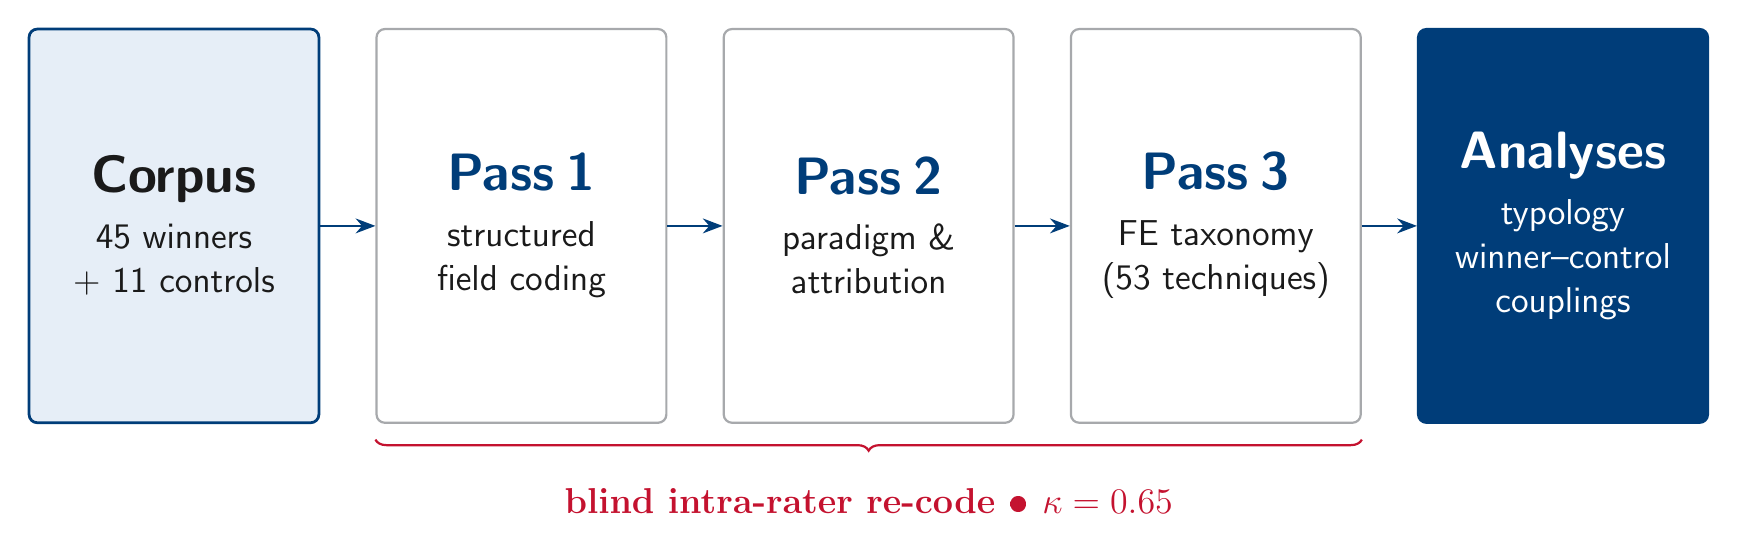
\begin{tikzpicture}[
  font=\fontsize{13}{16}\selectfont\sffamily,
  >={Stealth[length=2.5mm]}, node distance=7mm,
  box/.style={rectangle, rounded corners=3pt, draw=BCSilver, line width=0.8pt,
              fill=white, text=BCInk, align=center, inner sep=4pt,
              minimum height=50mm, minimum width=36mm, text width=34mm},
  io/.style={box, fill=BCLightBlue, draw=BCBlue, line width=1pt},
  result/.style={box, fill=BCBlue, text=white, draw=BCBlue},
  arr/.style={->, draw=BCBlue, line width=1pt},
]
\node[io] (corpus) {{\fontsize{19}{22}\selectfont\bfseries Corpus}\\[4pt]45 winners\\+ 11 controls};
\node[box, right=of corpus] (p1) {{\fontsize{19}{22}\selectfont\bfseries\color{BCBlue}Pass 1}\\[4pt]structured\\field coding};
\node[box, right=of p1] (p2) {{\fontsize{19}{22}\selectfont\bfseries\color{BCBlue}Pass 2}\\[4pt]paradigm \&\\attribution};
\node[box, right=of p2] (p3) {{\fontsize{19}{22}\selectfont\bfseries\color{BCBlue}Pass 3}\\[4pt]FE taxonomy\\(53 techniques)};
\node[result, right=of p3] (out) {{\fontsize{19}{22}\selectfont\bfseries Analyses}\\[4pt]typology\\winner--control\\couplings};
\draw[arr] (corpus) -- (p1);
\draw[arr] (p1) -- (p2);
\draw[arr] (p2) -- (p3);
\draw[arr] (p3) -- (out);
\draw[decorate, decoration={brace, amplitude=4pt, mirror}, draw=BCRed, line width=0.8pt]
  ([yshift=-2mm]p1.south west) -- ([yshift=-2mm]p3.south east);
\node[text=BCRed, font=\fontsize{13}{16}\selectfont\bfseries, below=7mm of p2.south]
  {blind intra-rater re-code \textbullet\ $\kappa = 0.65$};
\end{tikzpicture}%
}}
\figcap{Figure 1. Multi-pass coding workflow with a near-winner control group and reliability check.}
\end{posterblock}

% ---------- COLUMN BREAK ----------
\columnbreak

\begin{posterblock}{Analytical Framework}
No model is trained. The unit is one completed solution (no RMSE/accuracy). The framework:

\begin{itemize}[leftmargin=1.4em,itemsep=5pt,topsep=4pt]
  \item \textbf{Four paradigms:} ensemble-stacking, single-model-FE, lookup-exploit, problem-fit-NN.
  \item \textbf{Winner--control design:} paired FE comparison (sign test).
  \item \textbf{Coupling audit:} six folklore ``constraint$\rightarrow$strategy'' claims tested.
\end{itemize}

\vspace{0.4em}
\begin{callout}
\centering\large
Each winner is tested against a \textbf{near-winning control} from the \emph{same}
competition. That comparison isolates what distinguishes \emph{winning} from
merely strong play.
\end{callout}
\end{posterblock}

\begin{posterblock}{Implementation \& Tools}
\renewcommand{\arraystretch}{1.3}
\begin{tabular}{@{}>{\raggedright\arraybackslash}p{0.30\linewidth}>{\raggedright\arraybackslash}p{0.64\linewidth}@{}}
\toprule
\textbf{Component} & \textbf{Tools / Libraries} \\
\midrule
Language / env & Python 3.13, Poetry \\
Analysis       & pandas, numpy, Python standard library \\
Collection     & Kaggle API, requests + BeautifulSoup \\
Coding         & \texttt{anthropic} SDK + Claude Code (AI-assisted, researcher-directed) \\
Visualization  & matplotlib \\
\bottomrule
\end{tabular}
\end{posterblock}

\begin{posterblock}{Inside Winning Solutions}
Sized by how many of the 45 winners use each: a few models and \textbf{ensemble
stacking} dominate, while feature engineering is a long, varied tail.

\vspace{0.9em}

\includegraphics[width=\linewidth]{wordcloud_winning}

\vspace{1.1em}
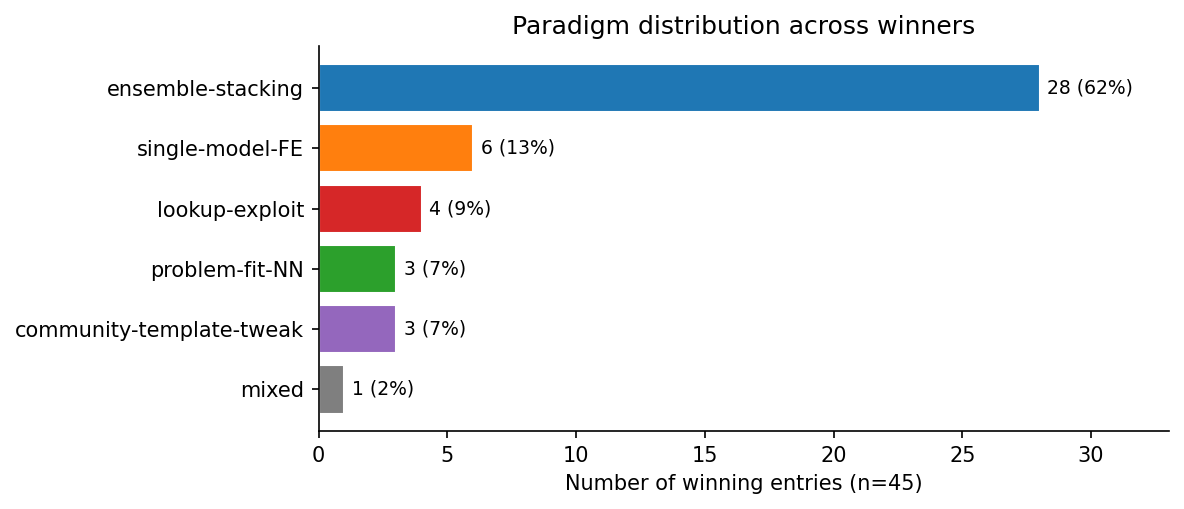
\includegraphics[width=\linewidth]{fig01_paradigm_distribution}
\figcap{Figure 2. Technique vocabulary (word size = winners using it) and the paradigm split.}
\end{posterblock}

% ---------- COLUMN BREAK ----------
\columnbreak

\begin{posterblock}{Results}
\textbf{FE does not cleanly separate winners from near-winners} ($n=11$, not significant);
only \emph{learned} features lean winner.

\vspace{0.4em}
\centerline{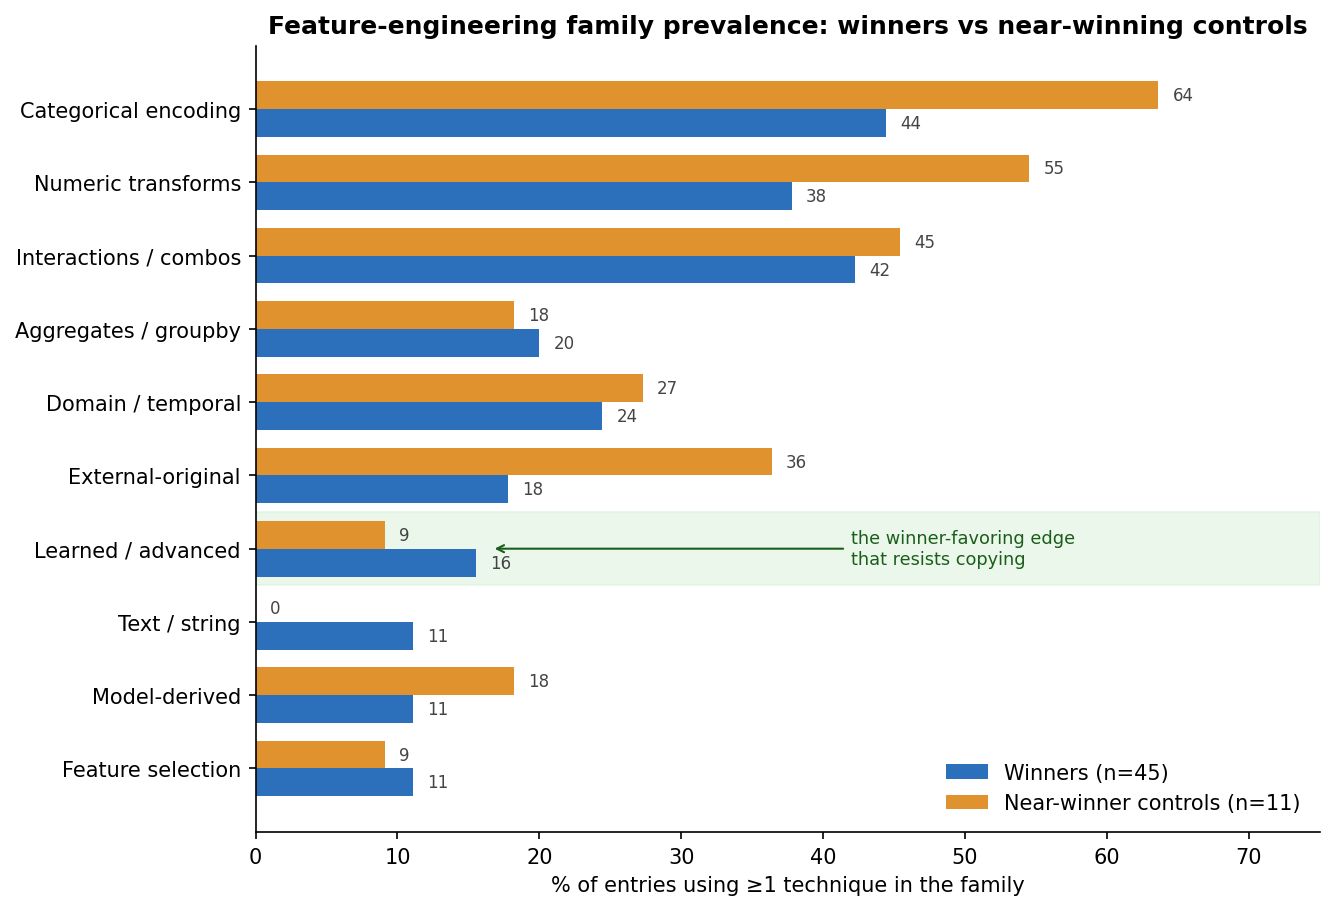
\includegraphics[width=0.86\linewidth]{fig05_fe_prevalence_winners_vs_controls}}
\figcap{Figure 3. FE-family prevalence, winners vs.\ near-winning controls.}

\vspace{0.5em}
\textbf{5 of 6 couplings aren't supported.} Only linear-stacker dominance holds, and it
just restates standard~ensembling.

\vspace{0.4em}
\centerline{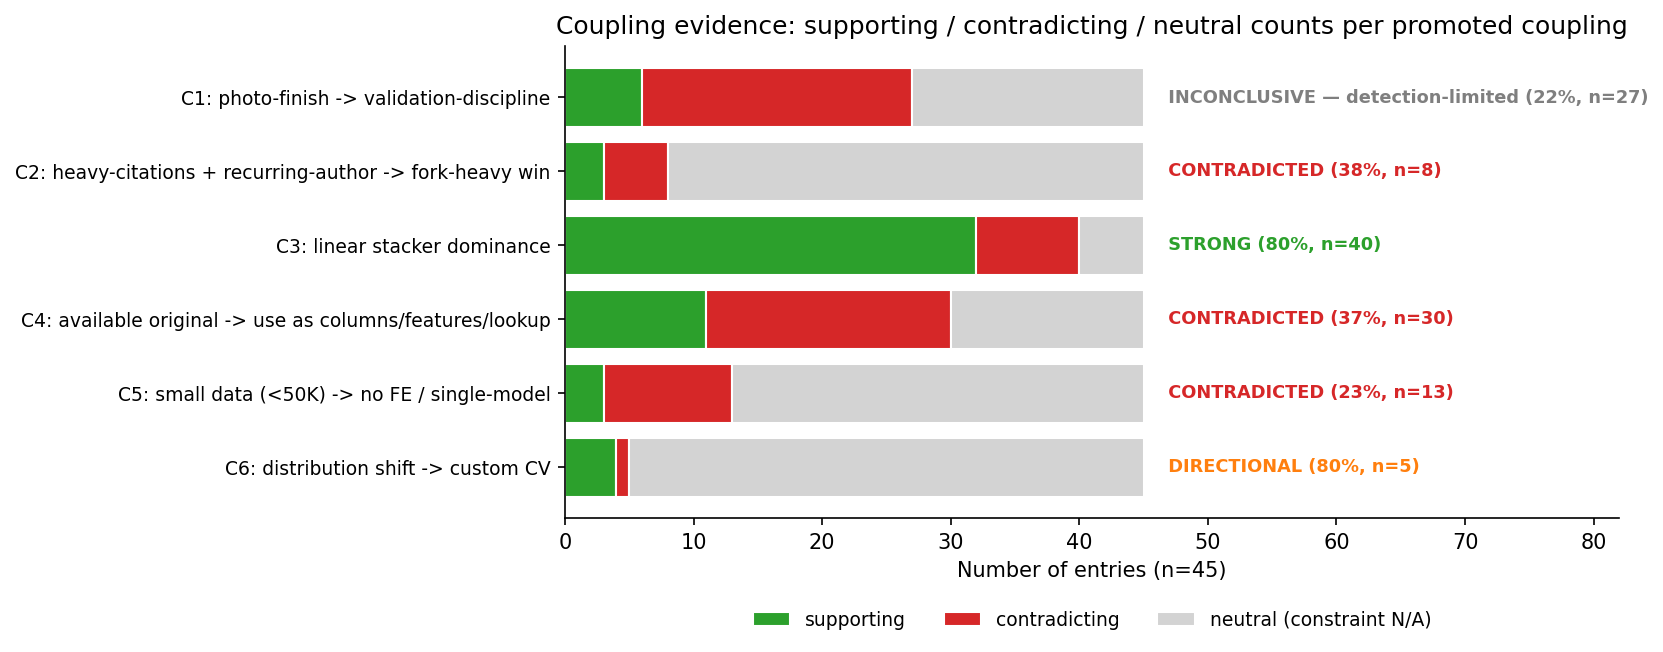
\includegraphics[width=0.86\linewidth]{fig02_coupling_evidence}}
\figcap{Figure 4. Coupling-evidence verdicts across the six promoted couplings.}
\end{posterblock}

\begin{posterblock}{Community Structure}
\textbf{A small recurring guild.} A few authors recur across winners and near-winners; some win, others mainly supply widely-cited techniques (originators vs.\ canonizers).

\vspace{0.3em}
\centerline{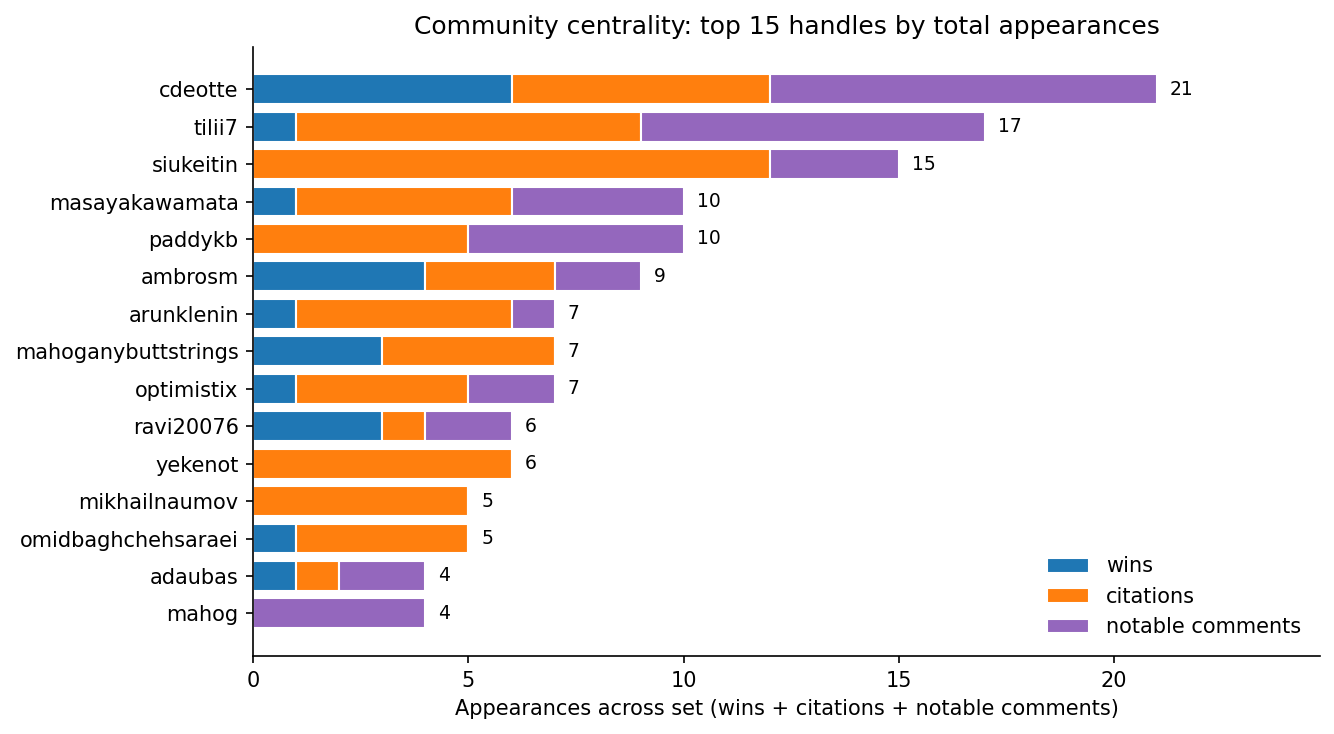
\includegraphics[width=\linewidth]{fig07_author_centrality}}
\figcap{Figure 5. Most-central community members, by wins + citations + notable comments.}
\end{posterblock}

\begin{posterblock}{Discussion \& Conclusions}
\textbf{Key Takeaways}
\begin{itemize}[leftmargin=1.4em,itemsep=6pt,topsep=4pt]
  \item Winning $\neq$ FE folklore: a small shared core, not elaborate craft.
  \item \textbf{Learned features:} the one edge that leans to~winners.
  \item The top is a \textbf{recurring guild} (45\% author overlap), partly about \emph{who competes}.
\end{itemize}

\vspace{0.4em}
\textbf{Limitations:} small $n$; synthetic-data corpus; intra-rater reliability; documentation-self-selection.

\vspace{0.3em}
\textbf{Future Work:} real-data Featured competitions; other platforms and modalities.
\end{posterblock}

\end{multicols}

% ---------- Full-width References + Acknowledgments band (ancillary) ----------
\vfill
\noindent
\begin{minipage}[t]{0.635\textwidth}
\begin{posterblock}{References}
\small
\begin{enumerate}[leftmargin=1.6em,itemsep=2pt,topsep=2pt]
  \item Caruana, R., \& Niculescu-Mizil, A. (2006). An empirical comparison of supervised learning algorithms. \textit{ICML}, 161--168.
  \item Gorishniy, Y., et al. (2021). Revisiting deep learning models for tabular data. \textit{NeurIPS 34}.
  \item Borisov, V., et al. (2024). Deep neural networks and tabular data: A survey. \textit{IEEE TNNLS, 35}(6).
  \item Makridakis, S., Spiliotis, E., \& Assimakopoulos, V. (2022). M5 accuracy competition: Results, findings, conclusions. \textit{Int.\ J.\ Forecasting, 38}(4).
  \item Merton, R.~K. (1968). The Matthew effect in science. \textit{Science, 159}(3810).
  \item Zhang, T., et al. (2023). OpenFE: Automated feature generation with expert-level performance. \textit{ICML}.
\end{enumerate}
\end{posterblock}
\end{minipage}
\hfill
\begin{minipage}[t]{0.345\textwidth}
\begin{posterblock}{Acknowledgments \& Contact}
The author thanks \textbf{Dr.~Pedro Albuquerque} for his guidance throughout CS\,495, and the
Bellevue College Computer Science program for supporting this capstone.

\vspace{0.4em}
\textbf{Contact:} kenneth.young@bellevuecollege.edu\\
\textbf{Code:} github.com/kennethyyoung/CS495-Mapping-Best-Empirical-Models
\end{posterblock}
\end{minipage}

% ---------- Footer band ----------
\vspace{0.6em}
\noindent
\begin{tikzpicture}
  \fill[BCBlue] (0,0) rectangle (\textwidth, 2cm);
  \fill[BCRed]  (0,2cm) rectangle (\textwidth, 2.25cm);
  \node[anchor=west] at (1cm, 1cm)
    {\color{BCDarkBlue}\bfseries\LARGE CS\,495 -- Data Science Project Practicum};
  \node[anchor=east] at (\textwidth-1cm, 1cm)
    {\color{BCDarkBlue}\LARGE Bellevue College \;\textbullet\; June 2026};
\end{tikzpicture}

\end{document}
